\documentclass{article}

\usepackage[utf8]{inputenc}
\usepackage[T1]{fontenc}
\usepackage[norsk,english]{babel}   %norsk først så engelsk, så engelsk blir prioritert
\usepackage{graphicx}
\usepackage{amsmath}
\usepackage{listings}
\usepackage{multicol}
\usepackage[margin=2.54cm]{geometry}
\usepackage{wrapfig}

%Definerer hyperlinker og dens farger
\usepackage{hyperref}
\hypersetup{
    colorlinks,
    citecolor=black,
    filecolor=black,
    linkcolor=blue,
    urlcolor=blue
}

%-----------------------------------

%Definerer farger til kodeeksemplene i PDF-en
\usepackage{color}

\definecolor{codegreen}{rgb}{0,0.6,0}
\definecolor{codegray}{rgb}{0.5,0.5,0.5}
\definecolor{codepurple}{rgb}{0.58,0,0.82}
\definecolor{backcolour}{rgb}{0.95,0.95,0.92}

\lstdefinestyle{mystyle}{
    backgroundcolor=\color{backcolour},
    commentstyle=\color{codegreen},
    keywordstyle=\color{magenta},
    numberstyle=\tiny\color{codegray},
    stringstyle=\color{codepurple},
    basicstyle=\footnotesize,
    breakatwhitespace=false,
    breaklines=true,
    captionpos=b,
    keepspaces=true,
    numbers=left,
    numbersep=5pt,
    showspaces=false,
    showstringspaces=false,
    showtabs=false,
    tabsize=2
}

\lstset{style=mystyle}

%------------------------------------

\setlength{\parindent}{0pt}
\setlength{\columnsep}{5mm} %column separation
\setlength{\columnsep}{10mm}

\setlength{\tabcolsep}{18pt}
\renewcommand{\arraystretch}{1.5}

\iffalse
If you want to change this temporarily, you can write:
\savegeometry{mydefaultgeometry}
\newgeometry{margin=3in}
And then later you can call:
\loadgeometry{mydefaultgeometry}
\fi

\begin{document}

\addtocounter{page}{0}

\title{Project 3 \\
      \large For the course FYS3150}
\date{\today \\
    \vspace{1mm}
    \large Week 40 - ??}

\author{Erik Grammeltvedt, Erlend Tiberg North and Alexandra Jahr Kolstad}

\maketitle

%\newpage

%------------Her starter skrivingen-----------------------------------------
\vspace{1cm}

\tableofcontents

\vspace{1cm}

%---------------------------------------
%\begin{multicols}{2}

\newpage
\clearpage

\textbf{Kommentarer fra project 1 på devilry:}

\begin{itemize}

\item Abstract: short motivation and presentation of the results and the findings \\

\item Introduction: you want to motive the reader about the problem and why you want solve it \\

\item Theory: explaining the theory behind the solution method and the problem \\

\item Method/implementation: how you implement the solution in order to fix/solve the problem \\

\item Results/graphs/tables: presenting the results \\

\item Discussion: Discussing the result from previous section \\

\item Conclusion: concluding the findings, your neutral opinion, etc… and future work \\

\item Appendix: How you derived your method, theory, etc… , altså utledning av ting i teori som ikke spesifikt er et bevis \\

\end{itemize}


Ting å gjøre for de ulike oppgavene:
\begin{itemize}

  \item 3a: beregne integralet, how many mesh points, lage et plott for å sjekke om grensene er passende å bruke \\

  \item 3b: finne grensene, erstatte Gauss-Legendre metoden med Laguerre polynomer, sammenligne med resultater fra a \\

  \item 3c: nå bruke brute force Monte Carlo, sammenligne resultatene med tidligere \\

  \item 3d: forbedre Monte Carlo med bruk av importance sampling, kommentere resultatene, lage en liste over tidene, sammenligne resultatene \\

  \item 3e: parallellisere koden fra 3d med openMPI eller MPI, kommenter resultatene (hovedsakelig i tiden brukt)

\end{itemize}


%----------Abstract-------------------------------
\vspace{1cm}

\section{Abstract} \label{sec:Abstract}

hensikt: tilnærme løsningen til integralet så best som mulig 5 pi**2 / 16**2 .

\begin{verbatim}

  


\end{verbatim}


%--------------Introduction------------------------------
\vspace{1cm}

\section{Introduction} \label{sec:Introduction}

All programs are found at our \href{https://github.com/Erikbgram/Fys3150}{GitHub-repository}. \\



%--------------- Theory ------------------------------------
\vspace{1cm}

\section{Theory} \label{sec:Theory}


  \begin{equation*} \label{eq:fullmatrixeq}
    \begin{bmatrix}
        d & a & 0 & \dots & 0 & 0 \\
        a & d & a & \dots & 0 & 0 \\
        0 & a & d & \dots & 0 & 0 \\
        \vdots & \vdots & \vdots & \ddots & \vdots & \vdots \\
        0 & 0 & 0 & a & d & a \\
        0 & 0 & 0 & 0 & a & d \\
    \end{bmatrix}
    \begin{bmatrix}
        u_1 \\
        u_2 \\
        u_3 \\
        \vdots \\
        u_{N-2} \\
        u_{N-1} \\
    \end{bmatrix}
      = \lambda
    \begin{bmatrix}
        u_1 \\
        u_2 \\
        u_3 \\
        \vdots \\
        u_{N-2} \\
        u_{N-1} \\
    \end{bmatrix}
  \end{equation*} \\



%--------------- Method ------------------------------------
\vspace{1cm}

\section{Method} \label{sec:Method}




%--------------------- Results ----------------------------------
\vspace{1cm}

\section{Results} \label{sec:Results}

  \textit{Our results are as shown in the \nameref{sec:Appendix}}. We also have \texttt{.txt}-files for all the raw data generated by the projects up on \href{https://github.com/Erikbgram/Fys3150}{GitHub}. \\

\begin{itemize}

  \item How many mesh points do you need before the results converges at the level of the third leading digit?

\end{itemize}

  Burde ha at lambda er 2 siden det gir best resultater, se plottet fra plot\_data.txt.


\iffalse

  \begin{figure}[ht]
  	\centering
    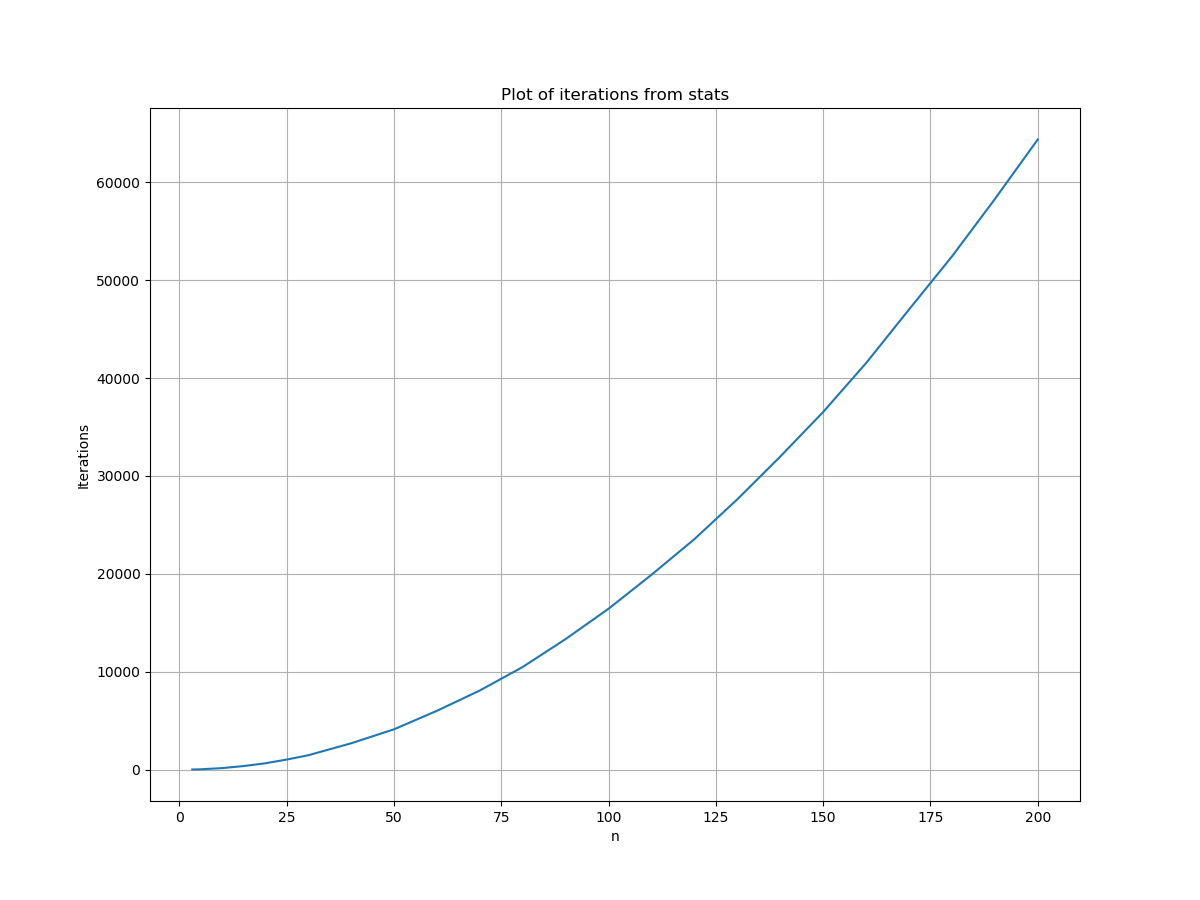
\includegraphics[width = 11cm]{iterations-stats.png}
    %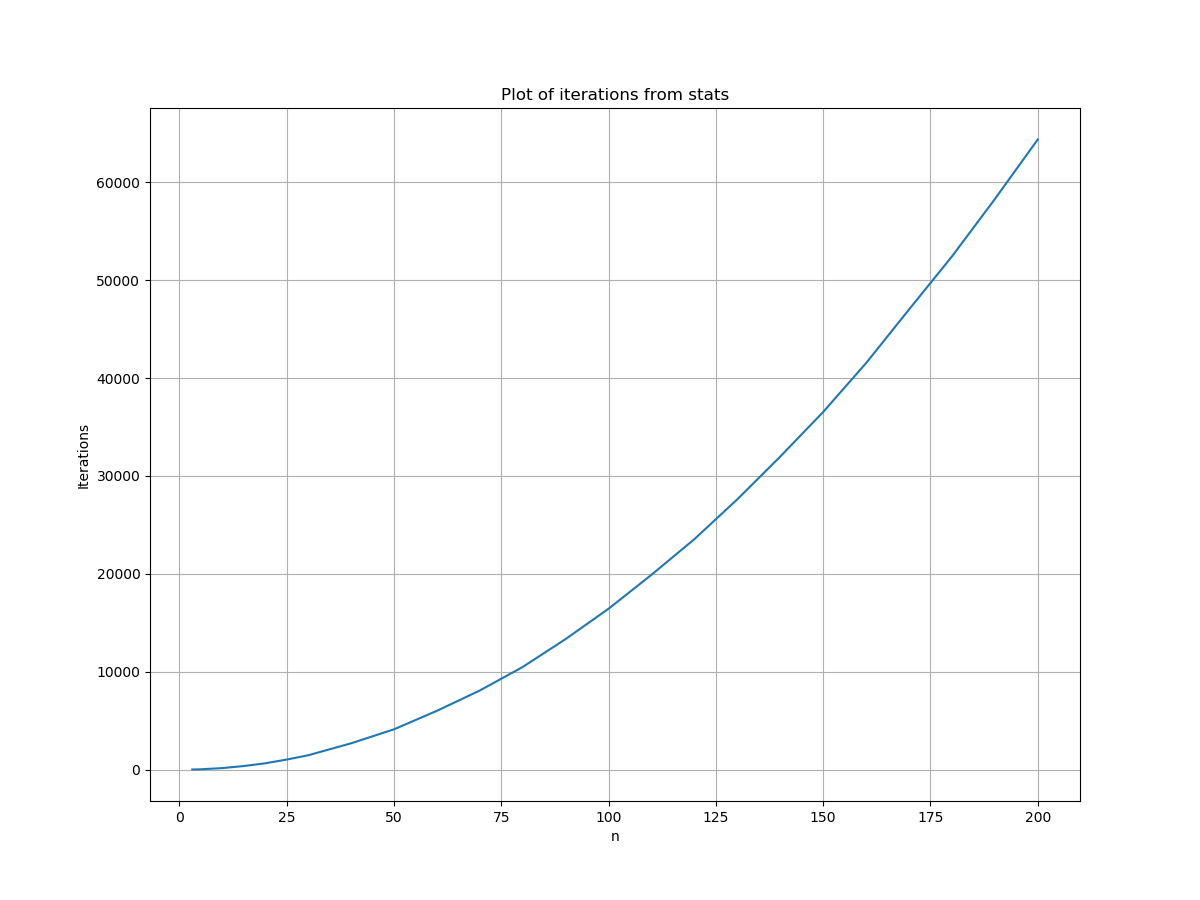
\includegraphics[width = \linewidth]{iterations-stats.png}
  	\caption{The plot of iterations for the Jacobi method as function of the dimension $n$ of the matrix \textbf{A}. }
    \label{fig:iterationspng}
  \end{figure}

  \begin{figure}[ht]
    \centering
    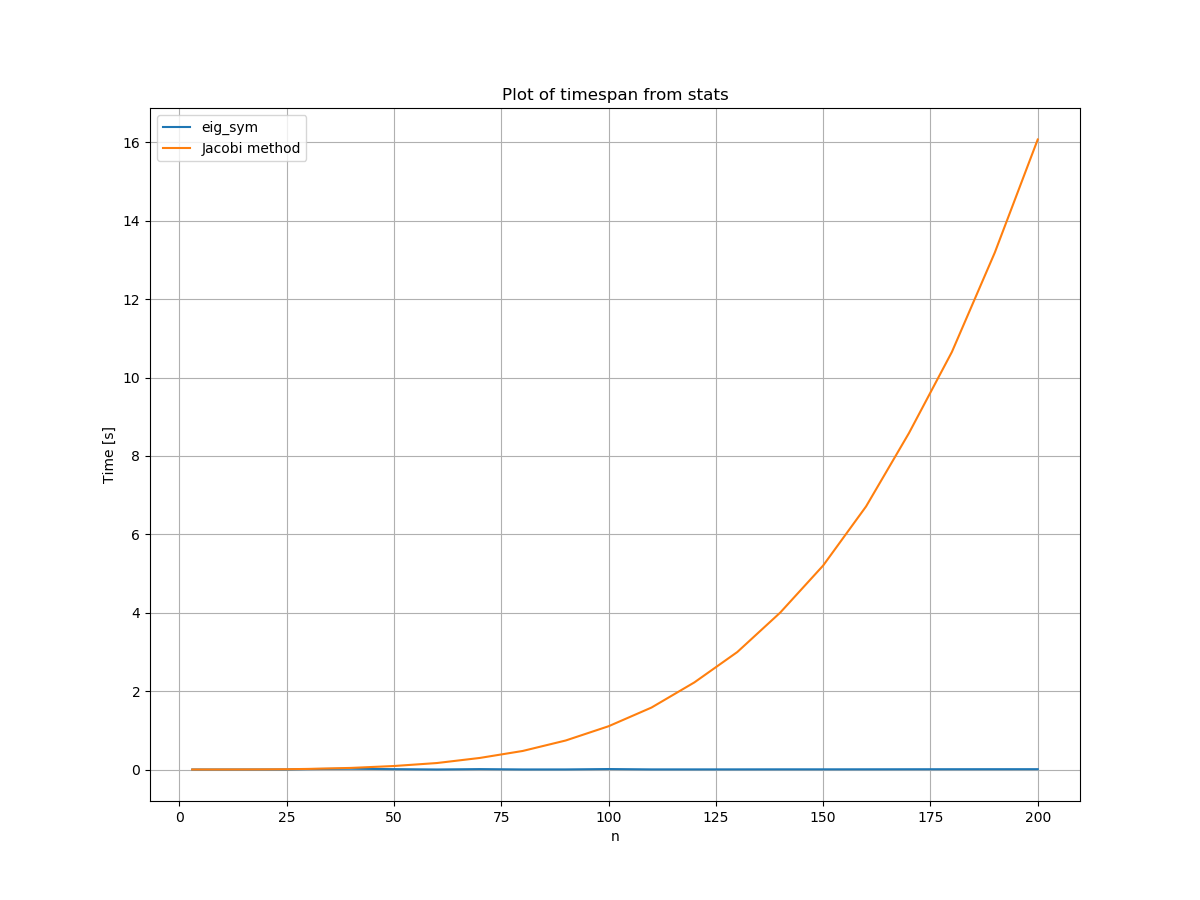
\includegraphics[width = 11cm]{timespan-stats.png}
    %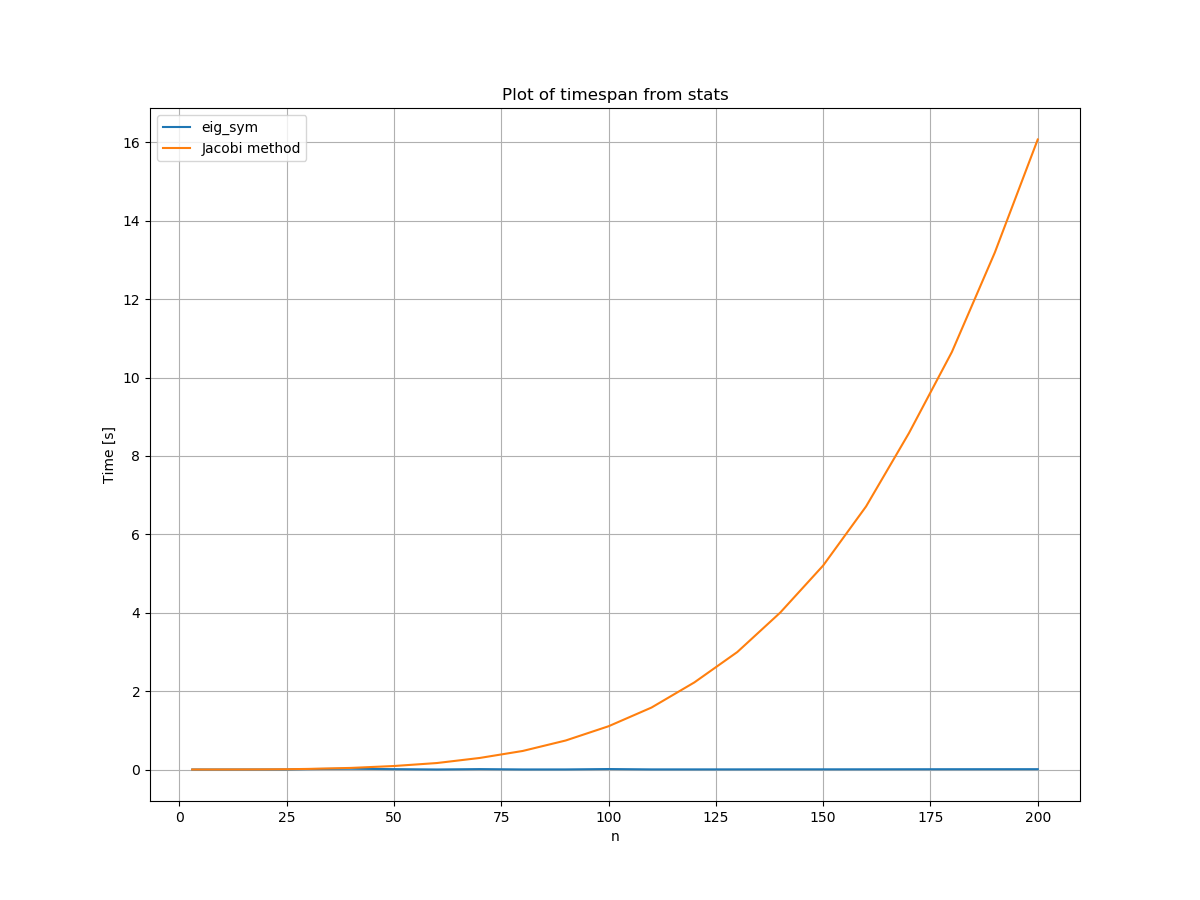
\includegraphics[width = \linewidth]{timespan-stats.png}
    \caption{The plot of the time the function \texttt{eig\_sym} from Armadillo uses and the time Jacobi method uses as functions of the dimension $n$ of the matrix \textbf{A}. }
    \label{fig:timespanpng}
  \end{figure}

\fi



%\vspace{3cm}


\iffalse
  \begin{table}[ht] \label{tab:exec_time}
    \centering
      \caption{Execution time for the two methods.}
      \vspace{2mm}
      \begin{tabular}{|c|c|c|}
        \hline
        $n$    &   Tridiagonal      &  LU-Decomposition  \\
        \hline \hline
        10   & $2.00\cdot10^{-7}$ & $3.17\cdot10^{-4}$ \\
        100  & $1,40\cdot10^{-6}$ & $1.40\cdot10^{-3}$ \\
        1000 & $1.44\cdot10^{-5}$ & $3.36\cdot10^{-2}$ \\
        \hline
      \end{tabular} \\
      \hspace{0pt}\\
  \end{table}
\fi

%--------------- Discussion ---------------------------------------
\vspace{1cm}

\section{Discussion} \label{sec:Discussion}




%---------------Conclusion and perspective---------------------------
\vspace{1cm}

\section{Conclusion and perspective} \label{sec:Conclusion}



%--------------Appendix---------------------------------------------
\vspace{1cm}

\section{Appendix} \label{sec:Appendix}






%\clearpage

%----------------Refrences----------------------------------------
\vspace{1cm}

\section{References} \label{sec:References}

\href{https://github.com/CompPhysics/ComputationalPhysics/blob/master/doc/Projects/2019/Project2/pdf/Project2.pdf}{Link to the PDF for Project 2}. \\

\href{https://github.com/Erikbgram/Fys3150}{Our GitHub-repository}. \\

\href{https://github.com/CompPhysics/ComputationalPhysics/blob/master/doc/Lectures/lectures2015.pdf}{Link to lecture slides in FYS3150 - Computational Physics}. \\

\href{http://arma.sourceforge.net/docs.html#eig_sym}{Offical Armadillo website for documentation of all contents in the library}. \\

\href{https://journals.aps.org/pra/pdf/10.1103/PhysRevA.48.3561}{Analytical results for specific oscillator frequencies}. \\





%----------------Slutten av dokumentet---------------------------------------



%\end{multicols}

\end{document}
